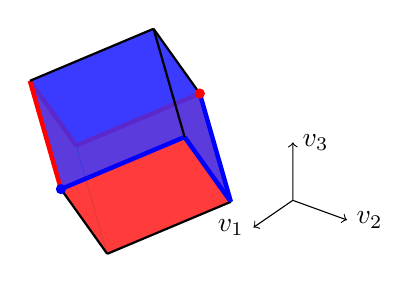
\begin{tikzpicture}%
	[x={(-0.587802cm, -0.404450cm)},
	y={(0.809005cm, -0.293947cm)},
	z={(0.000078cm, 0.866034cm)},
	scale=.850000,
	back/.style={thin, color=black!60},
	edge/.style={color=black, thick},
	sourceedge/.style={color=red, ultra thick},
	targetedge/.style={color=blue, ultra thick},
	facet/.style={fill=blue!95!black,fill opacity=0.800000},
	targetfacet/.style={fill=blue!80,fill opacity=0.800000},
	sourcefacet/.style={fill=red!80,fill opacity=0.800000},
	vertex/.style={inner sep=1pt,circle,draw=black,fill=black,thick},
	targetvertex/.style={inner sep=1pt,circle,draw=blue,fill=blue,thick},
	sourcevertex/.style={inner sep=1pt,circle,draw=red,fill=red,thick}]
	%
	%
	%% This TikZ-picture was produced with Sagemath version 10.0
	%% with the command: ._tikz_3d_in_3d and parameters:
	%% view = [-0.246900000000000, -0.484500000000000, -0.839200000000000]
	%% angle = 133.700000000000
	%% scale = 1
	%% edge_color = blue!95!black
	%% facet_color = blue!95!black
	%% opacity = 0.8
	%% vertex_color = green
	%% axis = False
	%%
	%% Coordinate of the vertices:
	%%
	\coordinate (-0.58824, 1.42857, -0.83333) at (-0.58824, 1.42857, -0.83333);
	\coordinate (0.58824, 1.42857, 0.83333) at (0.58824, 1.42857, 0.83333);
	\coordinate (1.76471, 0.00000, 0.00000) at (1.76471, 0.00000, 0.00000);
	\coordinate (0.58824, 0.00000, -1.66667) at (0.58824, 0.00000, -1.66667);
	\coordinate (-0.58824, -1.42857, -0.83333) at (-0.58824, -1.42857, -0.83333);
	\coordinate (-1.76471, 0.00000, 0.00000) at (-1.76471, 0.00000, 0.00000);
	\coordinate (-0.58824, 0.00000, 1.66667) at (-0.58824, 0.00000, 1.66667);
	\coordinate (0.58824, -1.42857, 0.83333) at (0.58824, -1.42857, 0.83333);
	%%
	%%
	%% Drawing edges in the back
	%%

	%%
	%%
	%% Drawing vertices in the back
	%%
	% \node[vertex] at (-0.58824, -1.42857, -0.83333)     {};
	%%
	%%
	\fill[targetfacet] (-0.58824, 0.00000, 1.66667) -- (0.58824, -1.42857, 0.83333) -- (-0.58824, -1.42857, -0.83333) -- (-1.76471, 0.00000, 0.00000) -- cycle {};
	\fill[sourcefacet] (-0.58824, 1.42857, -0.83333) -- (-1.76471, 0.00000, 0.00000) -- (-0.58824, -1.42857, -0.83333) -- (0.58824, 0.00000, -1.66667) -- cycle {};
	\fill[sourcefacet] (0.58824, 0.00000, -1.66667) -- (-0.58824, -1.42857, -0.83333) -- (0.58824, -1.42857, 0.83333) -- (1.76471, 0.00000, 0.00000) -- cycle {};


	\draw[edge,back] (0.58824, 0.00000, -1.66667) -- (-0.58824, -1.42857, -0.83333);
	\draw[back,sourceedge] (-0.58824, -1.42857, -0.83333) -- (-1.76471, 0.00000, 0.00000);
	\draw[back,sourceedge] (-0.58824, -1.42857, -0.83333) -- (0.58824, -1.42857, 0.83333);

	% %% Drawing the facets
	% %%
	\fill[sourcefacet] (0.58824, 0.00000, -1.66667) -- (-0.58824, 1.42857, -0.83333) -- (0.58824, 1.42857, 0.83333) -- (1.76471, 0.00000, 0.00000) -- cycle {};
	\fill[targetfacet] (0.58824, -1.42857, 0.83333) -- (1.76471, 0.00000, 0.00000) -- (0.58824, 1.42857, 0.83333) -- (-0.58824, 0.00000, 1.66667) -- cycle {};
	\fill[targetfacet] (-0.58824, 0.00000, 1.66667) -- (0.58824, 1.42857, 0.83333) -- (-0.58824, 1.42857, -0.83333) -- (-1.76471, 0.00000, 0.00000) -- cycle {};
	%%
	%%
	%% Drawing edges in the front
	%%
	\draw[targetedge] (-0.58824, 1.42857, -0.83333) -- (0.58824, 1.42857, 0.83333);
	\draw[edge] (-0.58824, 1.42857, -0.83333) -- (0.58824, 0.00000, -1.66667);
	\draw[targetedge] (-0.58824, 1.42857, -0.83333) -- (-1.76471, 0.00000, 0.00000);
	\draw[targetedge] (0.58824, 1.42857, 0.83333) -- (1.76471, 0.00000, 0.00000);
	\draw[edge] (0.58824, 1.42857, 0.83333) -- (-0.58824, 0.00000, 1.66667);
	\draw[edge] (1.76471, 0.00000, 0.00000) -- (0.58824, 0.00000, -1.66667);
	\draw[sourceedge] (1.76471, 0.00000, 0.00000) -- (0.58824, -1.42857, 0.83333);
	\draw[edge] (-1.76471, 0.00000, 0.00000) -- (-0.58824, 0.00000, 1.66667);
	\draw[edge] (-0.58824, 0.00000, 1.66667) -- (0.58824, -1.42857, 0.83333);
	%%
	%%
	% %% Drawing the vertices in the front
	% %%
	% \node[vertex] at (-0.58824, 1.42857, -0.83333)     {};
	% \node[vertex] at (0.58824, 1.42857, 0.83333)     {};
	\node[targetvertex] at (1.76471, 0.00000, 0.00000)     {};
	% \node[vertex] at (0.58824, 0.00000, -1.66667)     {};
	\node[sourcevertex] at (-1.76471, 0.00000, 0.00000)     {};
	% \node[vertex] at (-0.58824, 0.00000, 1.66667)     {};
	% \node[vertex] at (0.58824, -1.42857, 0.83333)     {};
	% %%
	% %%
	% %
	\begin{scope}[shift={(0,3,0)}]

		%axes
		\draw[->] (0, 0,0) -- (1, 0,0) node[anchor=east]{$v_1$};
		\draw[->] (0, 0,0) -- (0, 1,0) node[anchor=west]{$v_2$};
		\draw[->] (0, 0,0) -- (0, 0, 1) node[anchor=west]{$v_3$};
	\end{scope}

\end{tikzpicture}
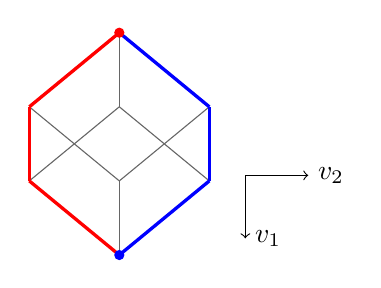
\begin{tikzpicture}%
	[
	x={(0.000000cm, -1.000000cm)},
	y={(1.000000cm, 0.000000cm)},
	z={(0.000000cm, 0.000000cm)},
	scale=.8,
	back/.style={thin, color=black!60},
	edge/.style={color=black, thick},
	sourceedge/.style={color=red, very thick},
	targetedge/.style={color=blue, very thick},
	facet/.style={fill=blue!95!black,fill opacity=0.800000},
	targetfacet/.style={fill=blue,fill opacity=0.600000},
	sourcefacet/.style={fill=red,fill opacity=0.600000},
	vertex/.style={inner sep=1pt,circle,draw=black,fill=black,thick},
	targetvertex/.style={inner sep=1pt,circle,draw=blue,fill=blue,thick},
	sourcevertex/.style={inner sep=1pt,circle,draw=red,fill=red,thick}]

\coordinate (-0.58824, 1.42857, -0.83333) at (-0.58824, 1.42857, -0.83333);
\coordinate (0.58824, 1.42857, 0.83333) at (0.58824, 1.42857, 0.83333);
\coordinate (1.76471, 0.00000, 0.00000) at (1.76471, 0.00000, 0.00000);
\coordinate (0.58824, 0.00000, -1.66667) at (0.58824, 0.00000, -1.66667);
\coordinate (-0.58824, -1.42857, -0.83333) at (-0.58824, -1.42857, -0.83333);
\coordinate (-1.76471, 0.00000, 0.00000) at (-1.76471, 0.00000, 0.00000);
\coordinate (-0.58824, 0.00000, 1.66667) at (-0.58824, 0.00000, 1.66667);
\coordinate (0.58824, -1.42857, 0.83333) at (0.58824, -1.42857, 0.83333);

\draw[edge,back] (-0.58824, 1.42857, -0.83333) -- (0.58824, 0.00000, -1.66667);
\draw[edge,back] (1.76471, 0.00000, 0.00000) -- (0.58824, 0.00000, -1.66667);
\draw[edge,back] (0.58824, 0.00000, -1.66667) -- (-0.58824, -1.42857, -0.83333);

\draw[edge,back] (0.58824, 1.42857, 0.83333) -- (-0.58824, 0.00000, 1.66667);
\draw[edge,back] (-1.76471, 0.00000, 0.00000) -- (-0.58824, 0.00000, 1.66667);
\draw[edge,back] (-0.58824, 0.00000, 1.66667) -- (0.58824, -1.42857, 0.83333);

\draw[back,sourceedge] (-0.58824, -1.42857, -0.83333) -- (-1.76471, 0.00000, 0.00000);
\draw[back,sourceedge] (-0.58824, -1.42857, -0.83333) -- (0.58824, -1.42857, 0.83333);
\draw[targetedge] (-0.58824, 1.42857, -0.83333) -- (0.58824, 1.42857, 0.83333);
\draw[targetedge] (-0.58824, 1.42857, -0.83333) -- (-1.76471, 0.00000, 0.00000);
\draw[targetedge] (0.58824, 1.42857, 0.83333) -- (1.76471, 0.00000, 0.00000);
\draw[sourceedge] (1.76471, 0.00000, 0.00000) -- (0.58824, -1.42857, 0.83333);
\node[targetvertex] at (1.76471, 0.00000, 0.00000)     {};
\node[sourcevertex] at (-1.76471, 0.00000, 0.00000)     {};
\begin{scope}[shift={(.5,2,0)}]
	\draw[->] (0, 0,0) -- (1, 0,0) node[anchor=west]{$v_1$};
	\draw[->] (0, 0,0) -- (0, 1,0) node[anchor=west]{$v_2$};
\end{scope}
\end{tikzpicture}
\begin{tikzpicture}%
	[scale=.8,
	back/.style={thin, color=black!60},
	edge/.style={color=black, thick},
	sourceedge/.style={color=red, very thick},
	targetedge/.style={color=blue, very thick},
	facet/.style={fill=blue!95!black,fill opacity=0.800000},
	targetfacet/.style={fill=blue,fill opacity=0.600000},
	sourcefacet/.style={fill=red,fill opacity=0.600000},
	vertex/.style={inner sep=1pt,circle,draw=black,fill=black,thick},
	targetvertex/.style={inner sep=1pt,circle,draw=blue,fill=blue,thick},
	sourcevertex/.style={inner sep=1pt,circle,draw=red,fill=red,thick}]
	\draw[edge] (0,-2) -- (0,1);
	\node[targetvertex] at (0,-2)     {};
	\node[sourcevertex] at (0,1)     {};

	\begin{scope}[shift={(1,-1)}]
		%axes
		\draw[->] (0, 0) -- ( 0,-1) node[anchor=west]{$v_1$};
	\end{scope}
\end{tikzpicture}
\vspace*{.8cm}

\pause
\centering
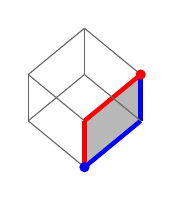
\begin{tikzpicture}%
	[	x={(0.000000cm, -1.000000cm)},
	y={(1.000000cm, 0.000000cm)},
	z={(0.000000cm, 0.000000cm)},
	scale=.5,
	back/.style={thin, color=black!60},
	edge/.style={color=black!60, thin},
	sourceedge/.style={color=red, ultra thick},
	targetedge/.style={color=blue, ultra thick},
	facet/.style={fill=black!35,fill opacity=0.800000},
	targetfacet/.style={fill=blue!80,fill opacity=0.800000},
	sourcefacet/.style={fill=red!80,fill opacity=0.800000},
	vertex/.style={inner sep=1pt,circle,draw=black,fill=black,thick},
	targetvertex/.style={inner sep=1pt,circle,draw=blue,fill=blue,thick},
	sourcevertex/.style={inner sep=1pt,circle,draw=red,fill=red,thick}]

\coordinate (-0.58824, 1.42857, -0.83333) at (-0.58824, 1.42857, -0.83333);
\coordinate (0.58824, 1.42857, 0.83333) at (0.58824, 1.42857, 0.83333);
\coordinate (1.76471, 0.00000, 0.00000) at (1.76471, 0.00000, 0.00000);
\coordinate (0.58824, 0.00000, -1.66667) at (0.58824, 0.00000, -1.66667);
\coordinate (-0.58824, -1.42857, -0.83333) at (-0.58824, -1.42857, -0.83333);
\coordinate (-1.76471, 0.00000, 0.00000) at (-1.76471, 0.00000, 0.00000);
\coordinate (-0.58824, 0.00000, 1.66667) at (-0.58824, 0.00000, 1.66667);
\coordinate (0.58824, -1.42857, 0.83333) at (0.58824, -1.42857, 0.83333);

\draw[edge,back] (0.58824, 0.00000, -1.66667) -- (-0.58824, -1.42857, -0.83333);
\draw[edge,back] (-0.58824, -1.42857, -0.83333) -- (-1.76471, 0.00000, 0.00000);
\draw[edge,back] (-0.58824, -1.42857, -0.83333) -- (0.58824, -1.42857, 0.83333);

\fill[facet] (0.58824, 0.00000, -1.66667) -- (-0.58824, 1.42857, -0.83333) -- (0.58824, 1.42857, 0.83333) -- (1.76471, 0.00000, 0.00000) -- cycle {};

\draw[targetedge] (-0.58824, 1.42857, -0.83333) -- (0.58824, 1.42857, 0.83333);
\draw[sourceedge] (-0.58824, 1.42857, -0.83333) -- (0.58824, 0.00000, -1.66667);
\draw[edge] (-0.58824, 1.42857, -0.83333) -- (-1.76471, 0.00000, 0.00000);
\draw[targetedge] (0.58824, 1.42857, 0.83333) -- (1.76471, 0.00000, 0.00000);
\draw[edge] (0.58824, 1.42857, 0.83333) -- (-0.58824, 0.00000, 1.66667);
\draw[sourceedge] (1.76471, 0.00000, 0.00000) -- (0.58824, 0.00000, -1.66667);
\draw[edge] (1.76471, 0.00000, 0.00000) -- (0.58824, -1.42857, 0.83333);
\draw[edge] (-1.76471, 0.00000, 0.00000) -- (-0.58824, 0.00000, 1.66667);
\draw[edge] (-0.58824, 0.00000, 1.66667) -- (0.58824, -1.42857, 0.83333);

\node[sourcevertex] at (-0.58824, 1.42857, -0.83333)     {};
\node[targetvertex] at (1.76471, 0.00000, 0.00000)     {};
\end{tikzpicture}
\qquad
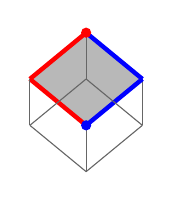
\begin{tikzpicture}%
	[x={(0.000000cm, -1.000000cm)},
	y={(1.000000cm, 0.000000cm)},
	z={(0.000000cm, 0.000000cm)},,
	scale=.5,
	back/.style={thin, color=black!60},
	edge/.style={color=black!60, thin},
	sourceedge/.style={color=red, ultra thick},
	targetedge/.style={color=blue, ultra thick},
	facet/.style={fill=black!35,fill opacity=0.800000},
	targetfacet/.style={fill=blue!80,fill opacity=0.800000},
	sourcefacet/.style={fill=red!80,fill opacity=0.800000},
	vertex/.style={inner sep=1pt,circle,draw=black,fill=black,thick},
	targetvertex/.style={inner sep=1pt,circle,draw=blue,fill=blue,thick},
	sourcevertex/.style={inner sep=1pt,circle,draw=red,fill=red,thick}]
%
\coordinate (-0.58824, 1.42857, -0.83333) at (-0.58824, 1.42857, -0.83333);
\coordinate (0.58824, 1.42857, 0.83333) at (0.58824, 1.42857, 0.83333);
\coordinate (1.76471, 0.00000, 0.00000) at (1.76471, 0.00000, 0.00000);
\coordinate (0.58824, 0.00000, -1.66667) at (0.58824, 0.00000, -1.66667);
\coordinate (-0.58824, -1.42857, -0.83333) at (-0.58824, -1.42857, -0.83333);
\coordinate (-1.76471, 0.00000, 0.00000) at (-1.76471, 0.00000, 0.00000);
\coordinate (-0.58824, 0.00000, 1.66667) at (-0.58824, 0.00000, 1.66667);
\coordinate (0.58824, -1.42857, 0.83333) at (0.58824, -1.42857, 0.83333);
%%
%%
%% Drawing edges in the back
%%

%%
%%
%% Drawing vertices in the back
%%
% \node[vertex] at (-0.58824, -1.42857, -0.83333)     {};
%%
%%
% \fill[targetfacet] (-0.58824, 0.00000, 1.66667) -- (0.58824, -1.42857, 0.83333) -- (-0.58824, -1.42857, -0.83333) -- (-1.76471, 0.00000, 0.00000) -- cycle {};
\fill[facet] (-0.58824, 1.42857, -0.83333) -- (-1.76471, 0.00000, 0.00000) -- (-0.58824, -1.42857, -0.83333) -- (0.58824, 0.00000, -1.66667) -- cycle {};
%  \fill[sourcefacet] (0.58824, 0.00000, -1.66667) -- (-0.58824, -1.42857, -0.83333) -- (0.58824, -1.42857, 0.83333) -- (1.76471, 0.00000, 0.00000) -- cycle {};


\draw[back,sourceedge] (0.58824, 0.00000, -1.66667) -- (-0.58824, -1.42857, -0.83333);
\draw[back,sourceedge] (-0.58824, -1.42857, -0.83333) -- (-1.76471, 0.00000, 0.00000);
\draw[edge,back] (-0.58824, -1.42857, -0.83333) -- (0.58824, -1.42857, 0.83333);

% %% Drawing the facets
% %%
% \fill[facet] (0.58824, 0.00000, -1.66667) -- (-0.58824, 1.42857, -0.83333) -- (0.58824, 1.42857, 0.83333) -- (1.76471, 0.00000, 0.00000) -- cycle {};
% \fill[facet] (0.58824, -1.42857, 0.83333) -- (1.76471, 0.00000, 0.00000) -- (0.58824, 1.42857, 0.83333) -- (-0.58824, 0.00000, 1.66667) -- cycle {};
%  \fill[targetfacet] (-0.58824, 0.00000, 1.66667) -- (0.58824, 1.42857, 0.83333) -- (-0.58824, 1.42857, -0.83333) -- (-1.76471, 0.00000, 0.00000) -- cycle {};
%%
%%
%% Drawing edges in the front
%%
\draw[edge] (-0.58824, 1.42857, -0.83333) -- (0.58824, 1.42857, 0.83333);
\draw[targetedge] (-0.58824, 1.42857, -0.83333) -- (0.58824, 0.00000, -1.66667);
\draw[targetedge] (-0.58824, 1.42857, -0.83333) -- (-1.76471, 0.00000, 0.00000);
\draw[edge] (0.58824, 1.42857, 0.83333) -- (1.76471, 0.00000, 0.00000);
\draw[edge] (0.58824, 1.42857, 0.83333) -- (-0.58824, 0.00000, 1.66667);
\draw[edge] (1.76471, 0.00000, 0.00000) -- (0.58824, 0.00000, -1.66667);
\draw[edge] (1.76471, 0.00000, 0.00000) -- (0.58824, -1.42857, 0.83333);
\draw[edge] (-1.76471, 0.00000, 0.00000) -- (-0.58824, 0.00000, 1.66667);
\draw[edge] (-0.58824, 0.00000, 1.66667) -- (0.58824, -1.42857, 0.83333);
%%
%%
% %% Drawing the vertices in the front
% %%
% \node[vertex] at (-0.58824, 1.42857, -0.83333)     {};
% \node[targetvertex] at (0.58824, 1.42857, 0.83333)     {};
% \node[targetvertex] at (1.76471, 0.00000, 0.00000)     {};
 \node[targetvertex] at (0.58824, 0.00000, -1.66667)     {};
 \node[sourcevertex] at (-1.76471, 0.00000, 0.00000)     {};
% \node[vertex] at (-0.58824, 0.00000, 1.66667)     {};
% \node[vertex] at (0.58824, -1.42857, 0.83333)     {};
% %%
% %%
% %
% \begin{scope}[shift={(0,3,0)}]
%
% 		%axes
% 		\draw[->] (0, 0,0) -- (1, 0,0) node[anchor=east]{$v_1$};
% 		\draw[->] (0, 0,0) -- (0, 1,0) node[anchor=west]{$v_2$};
% 		\draw[->] (0, 0,0) -- (0, 0, 1) node[anchor=west]{$v_3$};
% 	\end{scope}

\end{tikzpicture}
\qquad
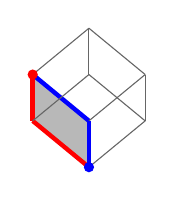
\begin{tikzpicture}%
	[x={(0.000000cm, -1.000000cm)},
	y={(1.000000cm, 0.000000cm)},
	z={(0.000000cm, 0.000000cm)},,
	scale=.5,
	back/.style={thin, color=black!60},
	edge/.style={color=black!60, thin},
	sourceedge/.style={color=red, ultra thick},
	targetedge/.style={color=blue, ultra thick},
	facet/.style={fill=black!35,fill opacity=0.800000},
	targetfacet/.style={fill=blue!80,fill opacity=0.800000},
	sourcefacet/.style={fill=red!80,fill opacity=0.800000},
	vertex/.style={inner sep=1pt,circle,draw=black,fill=black,thick},
	targetvertex/.style={inner sep=1pt,circle,draw=blue,fill=blue,thick},
	sourcevertex/.style={inner sep=1pt,circle,draw=red,fill=red,thick}]
%
\coordinate (-0.58824, 1.42857, -0.83333) at (-0.58824, 1.42857, -0.83333);
\coordinate (0.58824, 1.42857, 0.83333) at (0.58824, 1.42857, 0.83333);
\coordinate (1.76471, 0.00000, 0.00000) at (1.76471, 0.00000, 0.00000);
\coordinate (0.58824, 0.00000, -1.66667) at (0.58824, 0.00000, -1.66667);
\coordinate (-0.58824, -1.42857, -0.83333) at (-0.58824, -1.42857, -0.83333);
\coordinate (-1.76471, 0.00000, 0.00000) at (-1.76471, 0.00000, 0.00000);
\coordinate (-0.58824, 0.00000, 1.66667) at (-0.58824, 0.00000, 1.66667);
\coordinate (0.58824, -1.42857, 0.83333) at (0.58824, -1.42857, 0.83333);
%%
%%
%% Drawing edges in the back
%%

%%
%%
%% Drawing vertices in the back
%%
%%
%%
% \fill[targetfacet] (-0.58824, 0.00000, 1.66667) -- (0.58824, -1.42857, 0.83333) -- (-0.58824, -1.42857, -0.83333) -- (-1.76471, 0.00000, 0.00000) -- cycle {};
% \fill[facet] (-0.58824, 1.42857, -0.83333) -- (-1.76471, 0.00000, 0.00000) -- (-0.58824, -1.42857, -0.83333) -- (0.58824, 0.00000, -1.66667) -- cycle {};
 \fill[facet] (0.58824, 0.00000, -1.66667) -- (-0.58824, -1.42857, -0.83333) -- (0.58824, -1.42857, 0.83333) -- (1.76471, 0.00000, 0.00000) -- cycle {};


\draw[back,targetedge] (0.58824, 0.00000, -1.66667) -- (-0.58824, -1.42857, -0.83333);
\draw[edge,back] (-0.58824, -1.42857, -0.83333) -- (-1.76471, 0.00000, 0.00000);
\draw[back,sourceedge] (-0.58824, -1.42857, -0.83333) -- (0.58824, -1.42857, 0.83333);

% %% Drawing the facets
% %%
% \fill[facet] (0.58824, 0.00000, -1.66667) -- (-0.58824, 1.42857, -0.83333) -- (0.58824, 1.42857, 0.83333) -- (1.76471, 0.00000, 0.00000) -- cycle {};
% \fill[facet] (0.58824, -1.42857, 0.83333) -- (1.76471, 0.00000, 0.00000) -- (0.58824, 1.42857, 0.83333) -- (-0.58824, 0.00000, 1.66667) -- cycle {};
%  \fill[targetfacet] (-0.58824, 0.00000, 1.66667) -- (0.58824, 1.42857, 0.83333) -- (-0.58824, 1.42857, -0.83333) -- (-1.76471, 0.00000, 0.00000) -- cycle {};
%%
%%
%% Drawing edges in the front
%%
\draw[edge] (-0.58824, 1.42857, -0.83333) -- (0.58824, 1.42857, 0.83333);
\draw[edge] (-0.58824, 1.42857, -0.83333) -- (0.58824, 0.00000, -1.66667);
\draw[edge] (-0.58824, 1.42857, -0.83333) -- (-1.76471, 0.00000, 0.00000);
\draw[edge] (0.58824, 1.42857, 0.83333) -- (1.76471, 0.00000, 0.00000);
\draw[edge] (0.58824, 1.42857, 0.83333) -- (-0.58824, 0.00000, 1.66667);
\draw[targetedge] (1.76471, 0.00000, 0.00000) -- (0.58824, 0.00000, -1.66667);
\draw[sourceedge] (1.76471, 0.00000, 0.00000) -- (0.58824, -1.42857, 0.83333);
\draw[edge] (-1.76471, 0.00000, 0.00000) -- (-0.58824, 0.00000, 1.66667);
\draw[edge] (-0.58824, 0.00000, 1.66667) -- (0.58824, -1.42857, 0.83333);
%%
%%
% %% Drawing the vertices
% %%
\node[sourcevertex] at (-0.58824, -1.42857, -0.83333)     {};

% \node[vertex] at (-0.58824, 1.42857, -0.83333)     {};
% \node[targetvertex] at (0.58824, 1.42857, 0.83333)     {};
\node[targetvertex] at (1.76471, 0.00000, 0.00000)     {};
%  \node[vertex] at (0.58824, 0.00000, -1.66667)     {};
%  \node[targetvertex] at (-1.76471, 0.00000, 0.00000)     {};
% \node[vertex] at (-0.58824, 0.00000, 1.66667)     {};
% \node[vertex] at (0.58824, -1.42857, 0.83333)     {};
% %%
% %%
% %
% \begin{scope}[shift={(0,3,0)}]
%
% 		%axes
% 		\draw[->] (0, 0,0) -- (1, 0,0) node[anchor=east]{$v_1$};
% 		\draw[->] (0, 0,0) -- (0, 1,0) node[anchor=west]{$v_2$};
% 		\draw[->] (0, 0,0) -- (0, 0, 1) node[anchor=west]{$v_3$};
% 	\end{scope}

\end{tikzpicture}

\centering
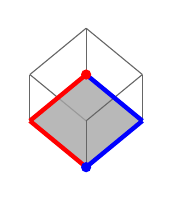
\begin{tikzpicture}%
	[x={(0.000000cm, -1.000000cm)},
	y={(1.000000cm, 0.000000cm)},
	z={(0.000000cm, 0.000000cm)},,
	scale=.5,
	back/.style={thin, color=black!60},
	edge/.style={color=black!60, thin},
	sourceedge/.style={color=red, ultra thick},
	targetedge/.style={color=blue, ultra thick},
	facet/.style={fill=black!35,fill opacity=0.800000},
	targetfacet/.style={fill=blue!80,fill opacity=0.800000},
	sourcefacet/.style={fill=red!80,fill opacity=0.800000},
	vertex/.style={inner sep=1pt,circle,draw=black,fill=black,thick},
	targetvertex/.style={inner sep=1pt,circle,draw=blue,fill=blue,thick},
	sourcevertex/.style={inner sep=1pt,circle,draw=red,fill=red,thick}]
%
\coordinate (-0.58824, 1.42857, -0.83333) at (-0.58824, 1.42857, -0.83333);
\coordinate (0.58824, 1.42857, 0.83333) at (0.58824, 1.42857, 0.83333);
\coordinate (1.76471, 0.00000, 0.00000) at (1.76471, 0.00000, 0.00000);
\coordinate (0.58824, 0.00000, -1.66667) at (0.58824, 0.00000, -1.66667);
\coordinate (-0.58824, -1.42857, -0.83333) at (-0.58824, -1.42857, -0.83333);
\coordinate (-1.76471, 0.00000, 0.00000) at (-1.76471, 0.00000, 0.00000);
\coordinate (-0.58824, 0.00000, 1.66667) at (-0.58824, 0.00000, 1.66667);
\coordinate (0.58824, -1.42857, 0.83333) at (0.58824, -1.42857, 0.83333);
%%
%%
%% Drawing edges in the back
%%

%%
%%
%% Drawing vertices in the back
%%
% \node[vertex] at (-0.58824, -1.42857, -0.83333)     {};
%%
%%
% \fill[targetfacet] (-0.58824, 0.00000, 1.66667) -- (0.58824, -1.42857, 0.83333) -- (-0.58824, -1.42857, -0.83333) -- (-1.76471, 0.00000, 0.00000) -- cycle {};
% \fill[facet] (-0.58824, 1.42857, -0.83333) -- (-1.76471, 0.00000, 0.00000) -- (-0.58824, -1.42857, -0.83333) -- (0.58824, 0.00000, -1.66667) -- cycle {};
%  \fill[facet] (0.58824, 0.00000, -1.66667) -- (-0.58824, -1.42857, -0.83333) -- (0.58824, -1.42857, 0.83333) -- (1.76471, 0.00000, 0.00000) -- cycle {};


\draw[edge,back] (0.58824, 0.00000, -1.66667) -- (-0.58824, -1.42857, -0.83333);
\draw[edge,back] (-0.58824, -1.42857, -0.83333) -- (-1.76471, 0.00000, 0.00000);
\draw[edge,back] (-0.58824, -1.42857, -0.83333) -- (0.58824, -1.42857, 0.83333);

% %% Drawing the facets
% %%
% \fill[facet] (0.58824, 0.00000, -1.66667) -- (-0.58824, 1.42857, -0.83333) -- (0.58824, 1.42857, 0.83333) -- (1.76471, 0.00000, 0.00000) -- cycle {};
\fill[facet] (0.58824, -1.42857, 0.83333) -- (1.76471, 0.00000, 0.00000) -- (0.58824, 1.42857, 0.83333) -- (-0.58824, 0.00000, 1.66667) -- cycle {};
%  \fill[targetfacet] (-0.58824, 0.00000, 1.66667) -- (0.58824, 1.42857, 0.83333) -- (-0.58824, 1.42857, -0.83333) -- (-1.76471, 0.00000, 0.00000) -- cycle {};
%%
%%
%% Drawing edges in the front
%%
\draw[edge] (-0.58824, 1.42857, -0.83333) -- (0.58824, 1.42857, 0.83333);
\draw[edge] (-0.58824, 1.42857, -0.83333) -- (0.58824, 0.00000, -1.66667);
\draw[edge] (-0.58824, 1.42857, -0.83333) -- (-1.76471, 0.00000, 0.00000);
\draw[targetedge] (0.58824, 1.42857, 0.83333) -- (1.76471, 0.00000, 0.00000);
\draw[targetedge] (0.58824, 1.42857, 0.83333) -- (-0.58824, 0.00000, 1.66667);
\draw[edge] (1.76471, 0.00000, 0.00000) -- (0.58824, 0.00000, -1.66667);
\draw[sourceedge] (1.76471, 0.00000, 0.00000) -- (0.58824, -1.42857, 0.83333);
\draw[edge] (-1.76471, 0.00000, 0.00000) -- (-0.58824, 0.00000, 1.66667);
\draw[sourceedge] (-0.58824, 0.00000, 1.66667) -- (0.58824, -1.42857, 0.83333);
%%
%%
% %% Drawing the vertices in the front
% %%
% \node[vertex] at (-0.58824, 1.42857, -0.83333)     {};
% \node[targetvertex] at (0.58824, 1.42857, 0.83333)     {};
\node[targetvertex] at (1.76471, 0.00000, 0.00000)     {};
%  \node[sourcevertex] at (0.58824, 0.00000, -1.66667)     {};
%  \node[targetvertex] at (-1.76471, 0.00000, 0.00000)     {};
 \node[sourcevertex] at (-0.58824, 0.00000, 1.66667)     {};
% \node[targetvertex] at (0.58824, -1.42857, 0.83333)     {};
% %%
% %%
% %
% \begin{scope}[shift={(0,3,0)}]
%
% 		%axes
% 		\draw[->] (0, 0,0) -- (1, 0,0) node[anchor=east]{$v_1$};
% 		\draw[->] (0, 0,0) -- (0, 1,0) node[anchor=west]{$v_2$};
% 		\draw[->] (0, 0,0) -- (0, 0, 1) node[anchor=west]{$v_3$};
% 	\end{scope}

\end{tikzpicture}
\qquad
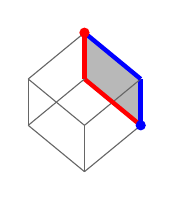
\begin{tikzpicture}%
	[x={(0.000000cm, -1.000000cm)},
	y={(1.000000cm, 0.000000cm)},
	z={(0.000000cm, 0.000000cm)},,
	scale=.5,
	back/.style={thin, color=black!60},
	edge/.style={color=black!60, thin},
	sourceedge/.style={color=red, ultra thick},
	targetedge/.style={color=blue, ultra thick},
	facet/.style={fill=black!35,fill opacity=0.800000},
	targetfacet/.style={fill=blue!80,fill opacity=0.800000},
	sourcefacet/.style={fill=red!80,fill opacity=0.800000},
	vertex/.style={inner sep=1pt,circle,draw=black,fill=black,thick},
	targetvertex/.style={inner sep=1pt,circle,draw=blue,fill=blue,thick},
	sourcevertex/.style={inner sep=1pt,circle,draw=red,fill=red,thick}]
%
\coordinate (-0.58824, 1.42857, -0.83333) at (-0.58824, 1.42857, -0.83333);
\coordinate (0.58824, 1.42857, 0.83333) at (0.58824, 1.42857, 0.83333);
\coordinate (1.76471, 0.00000, 0.00000) at (1.76471, 0.00000, 0.00000);
\coordinate (0.58824, 0.00000, -1.66667) at (0.58824, 0.00000, -1.66667);
\coordinate (-0.58824, -1.42857, -0.83333) at (-0.58824, -1.42857, -0.83333);
\coordinate (-1.76471, 0.00000, 0.00000) at (-1.76471, 0.00000, 0.00000);
\coordinate (-0.58824, 0.00000, 1.66667) at (-0.58824, 0.00000, 1.66667);
\coordinate (0.58824, -1.42857, 0.83333) at (0.58824, -1.42857, 0.83333);
%%
%%
%% Drawing edges in the back
%%

%%
%%
%% Drawing vertices in the back
%%
% \node[vertex] at (-0.58824, -1.42857, -0.83333)     {};
%%
%%
% \fill[targetfacet] (-0.58824, 0.00000, 1.66667) -- (0.58824, -1.42857, 0.83333) -- (-0.58824, -1.42857, -0.83333) -- (-1.76471, 0.00000, 0.00000) -- cycle {};
% \fill[facet] (-0.58824, 1.42857, -0.83333) -- (-1.76471, 0.00000, 0.00000) -- (-0.58824, -1.42857, -0.83333) -- (0.58824, 0.00000, -1.66667) -- cycle {};
%  \fill[facet] (0.58824, 0.00000, -1.66667) -- (-0.58824, -1.42857, -0.83333) -- (0.58824, -1.42857, 0.83333) -- (1.76471, 0.00000, 0.00000) -- cycle {};


\draw[edge,back] (0.58824, 0.00000, -1.66667) -- (-0.58824, -1.42857, -0.83333);
\draw[edge,back] (-0.58824, -1.42857, -0.83333) -- (-1.76471, 0.00000, 0.00000);
\draw[edge,back] (-0.58824, -1.42857, -0.83333) -- (0.58824, -1.42857, 0.83333);

% %% Drawing the facets
% %%
% \fill[facet] (0.58824, 0.00000, -1.66667) -- (-0.58824, 1.42857, -0.83333) -- (0.58824, 1.42857, 0.83333) -- (1.76471, 0.00000, 0.00000) -- cycle {};
% \fill[facet] (0.58824, -1.42857, 0.83333) -- (1.76471, 0.00000, 0.00000) -- (0.58824, 1.42857, 0.83333) -- (-0.58824, 0.00000, 1.66667) -- cycle {};
 \fill[facet] (-0.58824, 0.00000, 1.66667) -- (0.58824, 1.42857, 0.83333) -- (-0.58824, 1.42857, -0.83333) -- (-1.76471, 0.00000, 0.00000) -- cycle {};
%%
%%
%% Drawing edges in the front
%%
\draw[targetedge] (-0.58824, 1.42857, -0.83333) -- (0.58824, 1.42857, 0.83333);
\draw[edge] (-0.58824, 1.42857, -0.83333) -- (0.58824, 0.00000, -1.66667);
\draw[targetedge] (-0.58824, 1.42857, -0.83333) -- (-1.76471, 0.00000, 0.00000);
\draw[edge] (0.58824, 1.42857, 0.83333) -- (1.76471, 0.00000, 0.00000);
\draw[sourceedge] (0.58824, 1.42857, 0.83333) -- (-0.58824, 0.00000, 1.66667);
\draw[edge] (1.76471, 0.00000, 0.00000) -- (0.58824, 0.00000, -1.66667);
\draw[edge] (1.76471, 0.00000, 0.00000) -- (0.58824, -1.42857, 0.83333);
\draw[sourceedge] (-1.76471, 0.00000, 0.00000) -- (-0.58824, 0.00000, 1.66667);
\draw[edge] (-0.58824, 0.00000, 1.66667) -- (0.58824, -1.42857, 0.83333);
%%
%%
% %% Drawing the vertices in the front
% %%
% \node[sourcevertex] at (-0.58824, 1.42857, -0.83333)     {};
\node[targetvertex] at (0.58824, 1.42857, 0.83333)     {};
% \node[sourcevertex] at (1.76471, 0.00000, 0.00000)     {};
%  \node[sourcevertex] at (0.58824, 0.00000, -1.66667)     {};
 \node[sourcevertex] at (-1.76471, 0.00000, 0.00000)     {};
%  \node[targetvertex] at (-0.58824, 0.00000, 1.66667)     {};
% \node[targetvertex] at (0.58824, -1.42857, 0.83333)     {};
% %%
% %%
% %
% \begin{scope}[shift={(0,3,0)}]
%
% 		%axes
% 		\draw[->] (0, 0,0) -- (1, 0,0) node[anchor=east]{$v_1$};
% 		\draw[->] (0, 0,0) -- (0, 1,0) node[anchor=west]{$v_2$};
% 		\draw[->] (0, 0,0) -- (0, 0, 1) node[anchor=west]{$v_3$};
% 	\end{scope}

\end{tikzpicture}
\qquad
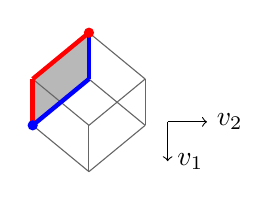
\begin{tikzpicture}%
	[x={(0.000000cm, -1.000000cm)},
	y={(1.000000cm, 0.000000cm)},
	z={(0.000000cm, 0.000000cm)},,
	scale=.5,
	back/.style={thin, color=black!60},
	edge/.style={color=black!60, thin},
	sourceedge/.style={color=red, ultra thick},
	targetedge/.style={color=blue, ultra thick},
	facet/.style={fill=black!35,fill opacity=0.800000},
	targetfacet/.style={fill=blue!80,fill opacity=0.800000},
	sourcefacet/.style={fill=red!80,fill opacity=0.800000},
	vertex/.style={inner sep=1pt,circle,draw=black,fill=black,thick},
	targetvertex/.style={inner sep=1pt,circle,draw=blue,fill=blue,thick},
	sourcevertex/.style={inner sep=1pt,circle,draw=red,fill=red,thick}]
%
\coordinate (-0.58824, 1.42857, -0.83333) at (-0.58824, 1.42857, -0.83333);
\coordinate (0.58824, 1.42857, 0.83333) at (0.58824, 1.42857, 0.83333);
\coordinate (1.76471, 0.00000, 0.00000) at (1.76471, 0.00000, 0.00000);
\coordinate (0.58824, 0.00000, -1.66667) at (0.58824, 0.00000, -1.66667);
\coordinate (-0.58824, -1.42857, -0.83333) at (-0.58824, -1.42857, -0.83333);
\coordinate (-1.76471, 0.00000, 0.00000) at (-1.76471, 0.00000, 0.00000);
\coordinate (-0.58824, 0.00000, 1.66667) at (-0.58824, 0.00000, 1.66667);
\coordinate (0.58824, -1.42857, 0.83333) at (0.58824, -1.42857, 0.83333);
%%
%%
%% Drawing edges in the back
%%

%%
%%
%% Drawing vertices in the back
%%
%%
%%
\fill[facet] (-0.58824, 0.00000, 1.66667) -- (0.58824, -1.42857, 0.83333) -- (-0.58824, -1.42857, -0.83333) -- (-1.76471, 0.00000, 0.00000) -- cycle {};
% \fill[facet] (-0.58824, 1.42857, -0.83333) -- (-1.76471, 0.00000, 0.00000) -- (-0.58824, -1.42857, -0.83333) -- (0.58824, 0.00000, -1.66667) -- cycle {};
%  \fill[facet] (0.58824, 0.00000, -1.66667) -- (-0.58824, -1.42857, -0.83333) -- (0.58824, -1.42857, 0.83333) -- (1.76471, 0.00000, 0.00000) -- cycle {};


\draw[edge,back] (0.58824, 0.00000, -1.66667) -- (-0.58824, -1.42857, -0.83333);
\draw[back,sourceedge] (-0.58824, -1.42857, -0.83333) -- (-1.76471, 0.00000, 0.00000);
\draw[back,sourceedge] (-0.58824, -1.42857, -0.83333) -- (0.58824, -1.42857, 0.83333);

% %% Drawing the facets
% %%
% \fill[facet] (0.58824, 0.00000, -1.66667) -- (-0.58824, 1.42857, -0.83333) -- (0.58824, 1.42857, 0.83333) -- (1.76471, 0.00000, 0.00000) -- cycle {};
% \fill[facet] (0.58824, -1.42857, 0.83333) -- (1.76471, 0.00000, 0.00000) -- (0.58824, 1.42857, 0.83333) -- (-0.58824, 0.00000, 1.66667) -- cycle {};
%  \fill[facet] (-0.58824, 0.00000, 1.66667) -- (0.58824, 1.42857, 0.83333) -- (-0.58824, 1.42857, -0.83333) -- (-1.76471, 0.00000, 0.00000) -- cycle {};
%%
%%
%% Drawing edges in the front
%%
\draw[edge] (-0.58824, 1.42857, -0.83333) -- (0.58824, 1.42857, 0.83333);
\draw[edge] (-0.58824, 1.42857, -0.83333) -- (0.58824, 0.00000, -1.66667);
\draw[edge] (-0.58824, 1.42857, -0.83333) -- (-1.76471, 0.00000, 0.00000);
\draw[edge] (0.58824, 1.42857, 0.83333) -- (1.76471, 0.00000, 0.00000);
\draw[edge] (0.58824, 1.42857, 0.83333) -- (-0.58824, 0.00000, 1.66667);
\draw[edge] (1.76471, 0.00000, 0.00000) -- (0.58824, 0.00000, -1.66667);
\draw[edge] (1.76471, 0.00000, 0.00000) -- (0.58824, -1.42857, 0.83333);
\draw[targetedge] (-1.76471, 0.00000, 0.00000) -- (-0.58824, 0.00000, 1.66667);
\draw[targetedge] (-0.58824, 0.00000, 1.66667) -- (0.58824, -1.42857, 0.83333);
%%
%%
% %% Drawing the vertices

% \node[targetvertex] at (-0.58824, -1.42857, -0.83333)     {};

% %%
% \node[sourcevertex] at (-0.58824, 1.42857, -0.83333)     {};
% \node[targetvertex] at (0.58824, 1.42857, 0.83333)     {};
% \node[sourcevertex] at (1.76471, 0.00000, 0.00000)     {};
%  \node[sourcevertex] at (0.58824, 0.00000, -1.66667)     {};
 \node[sourcevertex] at (-1.76471, 0.00000, 0.00000)     {};
%  \node[sourcevertex] at (-0.58824, 0.00000, 1.66667)     {};
 \node[targetvertex] at (0.58824, -1.42857, 0.83333)     {};
% %%
% %%
% %
% \begin{scope}[shift={(0,3,0)}]
%
% 		%axes
% 		\draw[->] (0, 0,0) -- (1, 0,0) node[anchor=east]{$v_1$};
% 		\draw[->] (0, 0,0) -- (0, 1,0) node[anchor=west]{$v_2$};
% 		\draw[->] (0, 0,0) -- (0, 0, 1) node[anchor=west]{$v_3$};
% 	\end{scope}
\begin{scope}[shift={(.5,2,0)}]
	\draw[->] (0, 0,0) -- (1, 0,0) node[anchor=west]{$v_1$};
	\draw[->] (0, 0,0) -- (0, 1,0) node[anchor=west]{$v_2$};
\end{scope}
\end{tikzpicture}
\\ \ \par